\chapter{Aufbau und Struktur M1 Modell} \label{M1Modell}
Beim M1-Modell handelt es sich um die direkte Darstellung der zu generierenden
Objekte. Dieses Modell wird direkt durch den Generator, siehe Abschnitt
\ref{Generator}, in Quellcode umgesetzt und dient somit als Grundlage des
zu generierenden Projektes. In dem in dieser Arbeit beschriebenen Generator, ist
es nicht vorgesehen ein vollständig lauffähiges Projekt zu erzeugen, aus diesem
Grund ist auch das M1-Modell nicht als vollständige Abbildung für das Projekt zu
verstehen. 

In dieser Arbeit, soll der Generator aus dem M1-Modell, lediglich eine möglichen
Grundstruktur für ein GWT-Projekt erzeugen. Das M1-Modell ist so angedacht das
alle Seiten eine eigenständige Klasse darstellen. Des Weiteren können einfache
Elemente, wie unter anderem Label und Textfelder den Seiten hinzugefügt werden.
Zu dem ist es möglich die Navigation zwischen den Seiten, beispielsweise mit
Hilfe eines Menüs, in das Modell mit ein zu bringen. 

Durch die Verwendung eines Profils, sind in dem M1-Modell keine Assoziationen
zu sehen. Dies sorg dafür das keine Verbindung zwischen den einzelnen Seiten zu
sehen ist. Die Navigation wird ausschließlich über die Properties der
Navigation Elemente, hier mit \texttt{viewNavigationObject} benannt. Dies
erschwert das Erkennen der Navigation, sorgt allerding dafür das Unabhängigkeit
der Seiten untereinander gut zu erkennen ist.

\section{Projetaufbau}
Wenn ein neues Projekt angelegt wird muss in den Properties des M1-Modelles
neben der Angabe des Profils, ein Name definiert werden. Dieser Name stellt
später den Hauptpaketnamen des GWT-Projektes da und legt somit den Grundstein
für die Paketstruktur (siehe Abbildung \ref{Fig:mainpackage}).

\begin{figure}[htbp]
\begin{center}
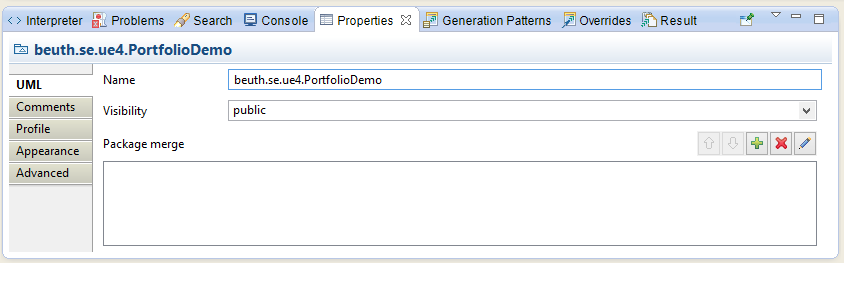
\includegraphics[width=0.8\textwidth]{./img/ProjectPackage.png}
\caption{Name des Modelles und gleichzeitig Hauptpakte des
GWT-Projekts}\label{Fig:mainpackage}
\end{center}
\end{figure}

\newpage
\section{Klassenaufbau}
Die Einfachsten Elemente in dem Modell sind \texttt{ViewImpl}-Klassen. ein
Beispiel dafür ist in Abbildung \ref{Fig:viewimpl} zu sehen. Für jede dieser
Klassen-Objekte, werden durch den Generator, alle notwendigen Dateien erzeugt
die für den späteren Aufruf, der Seite, notwendig sind.

\begin{figure}[htbp]
\begin{center}
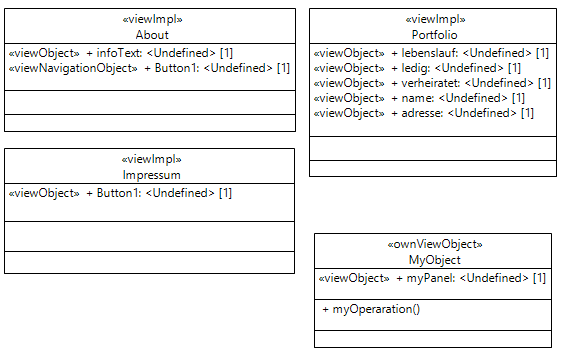
\includegraphics[width=1.0\textwidth]{./img/GWT-Model-Views-alg.png}
\caption{\texttt{ViewImpl}-Klassen zur Erzeugung von Seiten
für den Webauftritt.}\label{Fig:viewimpl}
\end{center}
\end{figure}

GWT bietet, unter Verwendung von Gin, eine einfache Möglichkeit Seiten
auszutauschen. Um dieses Verfahren mit zu generieren wurde sich dazu
entschlossen, neben der Standardgenerierung von Seiten, eine zusätzliche
Methode einzubauen. Diese Methode bietet die Möglichkeit beliebig viele
alternativ Seiten für eine Ansicht im Webauftritt zu erzeugen (siehe Abbildung
\ref{Fig:viewInterface}).Dieses Möglichkeit ist unter anderem für Testzwecke
gedacht.

\begin{figure}[htbp]
\begin{center}
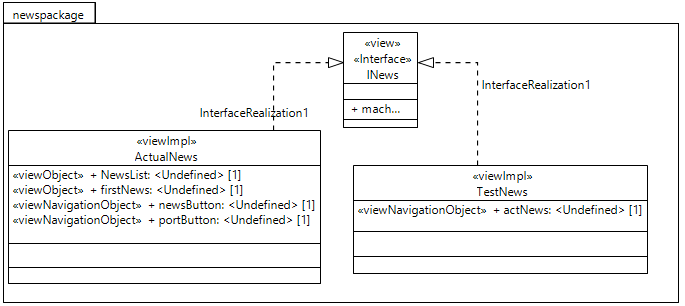
\includegraphics[width=1.0\textwidth]{./img/GWT-Model-Views-interface.png}
\caption{Ein Beispiel für die Verwendung der \texttt{ViewInterface}-Klassen
um mit Hilfe einer Vielzahl \texttt{ViewImpl}-Klassen
eine Austauschbare Ansicht zu erzeugen.}\label{Fig:viewInterface}
\end{center}
\end{figure} 

Bei dem, in Abbildung \ref{Fig:viewInterface}, gezeigtem M1-Model Ausschnitt.
wird anderes als im allgemeinen Fall (siehe Abbildung  \ref{Fig:viewimpl}) nicht
die komplette Struktur zweimal erzeugt. Die \grqq{}Name\grqq{}Activity.java,
\grqq{}Name\grqq{}Place.java und \grqq{}Name\grqq{}View.java Klassen, werden
hierbei nur einmal für das Interface und die \grqq{}Name\grqq{}ViewImpl.java und
\grqq{}Name\grqq{}ViewImpl.ui.xml Dateien werden für jede
\texttt{ViewImpl}-Klassen generiert. 

Darüber hinaus ist ein Abbildung \ref{Fig:viewInterface} zu sehen, das es
möglich ist Elemente in Paketen zu verpacken, auf diese Weise wird es
ermöglicht die zu generierenden Dateien zu gruppieren. 

\newpage
Das Letzte Klassenkonstrukt, sind die sogenannten
\texttt{PermanentView}-Elemente, diese sind dazu gedacht um zum Beispiel Menüs
zu erzeugen. Dies haben die Eigenschaft das sie auf allen Seiten zur Verfügung
stehen und nicht mehrfach generiert werden sollen.

\begin{figure}[htbp]
\begin{center}
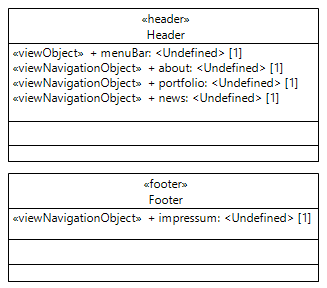
\includegraphics[width=0.55\textwidth]{./img/Header_Footer.png}
\caption{\texttt{PermanentView}-Elemente am Beispiel
eines Header, mit Menu, und eines Footers.}\label{Fig:headerFooter}
\end{center}
\end{figure} 

\newpage
\section{Seitenaufbau}
Je nach Art der Seite muss zuerst deferiert werden, um was für einen Typ von
Seite es sich handelt. In Abbildung \ref{Fig:SideProp} ist ein Beispiel dafür
zu sehen, hier ist eine \texttt{ViewImpl} und ein \texttt{Header}, eine
spezialisierte Version der \texttt{PermanentView}, zu sehen. Wichtig ist hier
die "`concreteBinding"' Eigenschaft, hier kann bei Verwendung eines
separaten Interfaces festgelegt werden, ob diese Klasse eingebunden werden soll
oder nicht. Diese Einstellung kann später im Quellecode weiter angepasst werden.

\begin{figure}[htbp]
\begin{center}
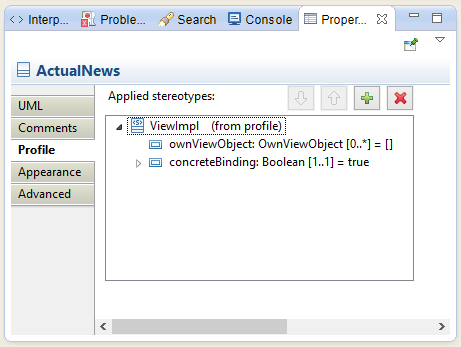
\includegraphics[width=0.8\textwidth]{./img/Prop-ViewImp.png}
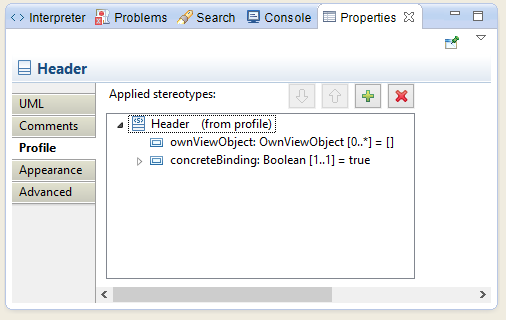
\includegraphics[width=0.8\textwidth]{./img/Prop-Header.png}
\caption{Definition der Stereotypen einer Klassen, oben
eine \texttt{ViewImpl} Definition und unten ein
\texttt{Header}}\label{Fig:SideProp}
\end{center}
\end{figure} 

Um deine Seite mit Inhalten zu befüllen, können \texttt{ViewObject}s und 
\texttt{ViewNavigationObject}s als Attribute hinzugefügt werden.

Bei \texttt{ViewObject}-Elementen können die in Abbildung \ref{Fig:ViewProp}
dargestellten Eigenschaften verändert werden.

\begin{figure}[htbp]
\begin{center}
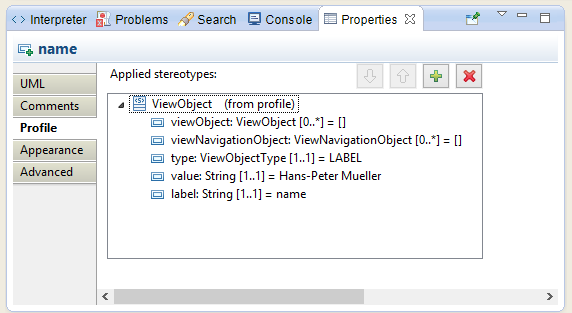
\includegraphics[width=0.8\textwidth]{./img/Prop-ViewObjects.png}
\caption{Eigenschaften eines \texttt{ViewObject}-Elementes }\label{Fig:ViewProp}
\end{center}
\end{figure} 

Bei \texttt{ViewNavigationObject}-Elementen können die in Abbildung
\ref{Fig:ViewNavProp} dargestellten Eigenschaften verändert werden. Hier ist
vor allem die letzte Eigenschaft "`goToView"' zu beachten, welche angibt wohin
dieses navigieren soll.

\begin{figure}[htbp]
\begin{center}
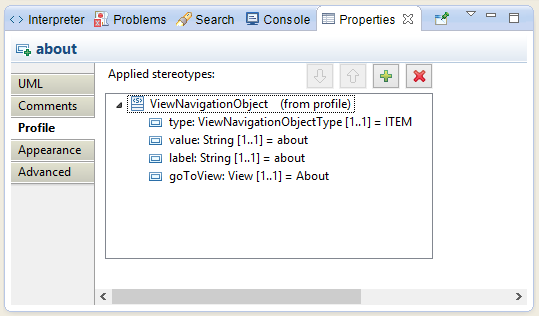
\includegraphics[width=0.8\textwidth]{./img/Prop-ViewNavigationObjects.png}
\caption{Eigenschaften eines \texttt{ViewNavigationObject}-Elementes
}\label{Fig:ViewNavProp}
\end{center}
\end{figure}
